\section*{Le déroulement de la partie} \label{sec:tourDeJeu}
\addcontentsline{toc}{section}{Le déroulement de la partie}
La partie se déroule en 15 manches, durant lesquelles chaque joueur va jouer un tour.

\subsection*{Le tour d'un joueur} \label{sec:tourDeJoueur}
\addcontentsline{toc}{subsection}{Le tour d'un joueur}
Le tour de jeu se divise en 3 phases successives, où le joueur :
\subsubsection*{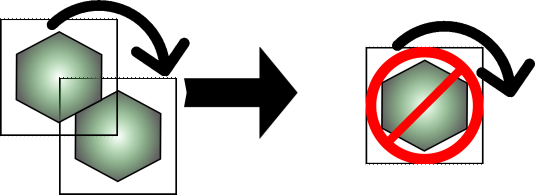
\includegraphics[scale=1]{icones/phase1} \\ Peut retourner deux tuiles}
Durant cette phase \textbf{facultative}, le joueur peut retourner deux \tuilesActives sur leur face \textit{bloquée}. Dans ce cas, il retourne une \tuileBloquee sur sa face \textit{active}.

\subsubsection*{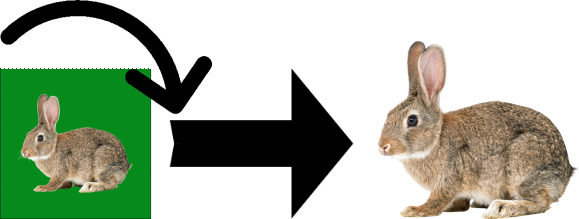
\includegraphics[scale=1]{icones/phase2} \\ Doit jouer une tuile}
Durant cette phase \textbf{obligatoire},
\begin{enumerate}
\item le joueur choisit une \tuileActive et la retourne sur sa face \textit{bloquée},
\item puis il joue l'action correspondante, en appliquant le multiplicateur associé.
\item Tous les joueurs retournent cette tuile et une autre
\end{enumerate}

\acompleter{EXEMPLE}
\subsubsection*{
\includegraphics[scale=1]{icones/phase3} \\ Peut jouer une carte}
Durant cette phase \textbf{facultative}, le joueur peut jouer une carte de sa main.

Une fois que le joueur a joué son tour, c'est au tour du joueur à sa gauche. Une fois que tous les joueurs ont joué leur tour, passer à l'étape de fin de manche.

\subsection*{La fin de la manche} \label{sec:finDeManche}
\addcontentsline{toc}{subsection}{La fin de la manche}
Pour marquer la fin de la manche, déplacer le \compteurManche d'une case et appliquer l'effet:
\begin{itemize}
\item 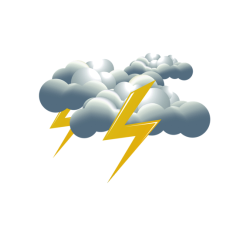
\includegraphics[scale=0.8]{jetonsMeteo/jetonEclair}: retournez toutes vos tuiles sur la face \textit{active}, sauf une sur sa face \textit{bloquee}
\item 
\includegraphics[scale=0.8]{jetonsMeteo/jetonTonnerre}: écartez définitivement une de vos tuiles
\item 
\includegraphics[scale=0.8]{jetonsMeteo/jetonSoleil}: profitez d'un tour de répit, rien ne se passe
\item 
\includegraphics[scale=0.8]{jetonsMeteo/jetonVent}: choisissez entre donner une carte à votre voisin de gauche ou perdre \textbf{3 points}
\item 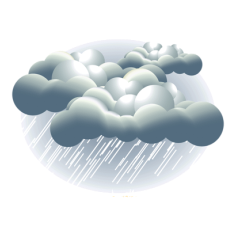
\includegraphics[scale=0.8]{jetonsMeteo/jetonPluie}: choisissez entre diminuer de 1 un des multiplicateur ou perdre \textbf{3 points}
\end{itemize}
\subsubsection*{}
